\section{胶片与成像管道}\label{sec:胶片与成像管道}
相机中胶片或传感器类型对入射光转换为图像中颜色的方式具有戏剧性影响。
在pbrt中,类\refvar{Film}{}在模拟相机中对传感设备建模。
在为每条相机光线求得辐亮度后,\refvar{Film}{}的实现
决定了样本对胶片平面上的相机光线起始点周围像素的贡献并更新其图像表示。
当主渲染循环退出时,\refvar{Film}{}将最终图像写入文件。

对于真实相机模型,\refsub{相机测量方程}介绍了测量方程,
它描述了相机中的传感器怎样度量一段时间内到达传感器区域上的能量大小。
对于更简单的相机模型,我们可将传感器视作度量某段时间内一小片区域上的平均辐亮度。
选择采用哪种度量的影响被封装在\refvar[GenerateRayDifferential]{Camera::GenerateRayDifferential}{()}为
光线返回的权重中。因此,\refvar{Film}{}的实现
可在不考虑这些变化的情况下处理,只需用这些权重缩放提供的辐亮度。

本节介绍了单个\refvar{Film}{}实现,它将像素重建方程应用于计算最终像素值。
对于基于物理的渲染器,通常最好是把结果图像存于浮点图像格式。
这样做在如何使用输出方面比起用8位无符号整数值的传统图像格式提供了更多的灵活性;
浮点格式避免了将图像量化为8位时造成的大量信息损失。

为了在现代显示设备上显示这样的图像,有必要将这些浮点像素值映射为离散值。
例如,计算机监视器通常希望每个像素的颜色由一个RGB颜色三元组描述,
而不是用任意的光谱功率分布。因此通用基函数系数描述的光谱在能显示之前必须转化为RGB表示。
一个相关问题是,比起许多真实世界场景中出现的范围,
显示器具有小得多的可显示辐亮度值范围。因此,像素值必须
以让最终显示的图像看起来尽可能接近其在无限制的理想显示设备上的样子的方式映射到可显示的范围。
这些问题是通过研究\keyindex{色调映射}{tone mapping}{}来解决的;
“扩展阅读”一节有关于该话题的更多信息。

\subsection{胶片类}\label{sub:胶片类}
\refvar{Film}{}定义在文件\href{https://github.com/mmp/pbrt-v3/blob/master/src/core/film.h}{\ttfamily core/film.h}
和\href{https://github.com/mmp/pbrt-v3/blob/master/src/core/film.cpp}{\ttfamily core/film.cpp}中。
\begin{lstlisting}
`\initcode{Film Declarations}{=}\initnext{FilmDeclarations}`
class `\initvar{Film}{}` {
public:
    `\refcode{Film Public Methods}{}`
    `\refcode{Film Public Data}{}`
private:
    `\refcode{Film Private Data}{}`
    `\refcode{Film Private Methods}{}`
};
\end{lstlisting}
\begin{lstlisting}
`\initcode{Film Public Methods}{=}`
`\refvar{Film}{}`(const `\refvar{Point2i}{}` &resolution, const `\refvar{Bounds2f}{}` &cropWindow,
    std::unique_ptr<`\refvar{Filter}{}`> filter,
    `\refvar{Float}{}` diagonal, const std::string &filename, `\refvar{Float}{}` scale);
`\refvar{Bounds2i}{}` `\refvar{GetSampleBounds}{}`() const;
`\refvar{Bounds2f}{}` `\refvar{GetPhysicalExtent}{}`() const;
std::unique_ptr<`\refvar{FilmTile}{}`> `\refvar{GetFilmTile}{}`(const `\refvar{Bounds2i}{}` &sampleBounds);
void `\refvar{MergeFilmTile}{}`(std::unique_ptr<`\refvar{FilmTile}{}`> tile);
void `\refvar{SetImage}{}`(const `\refvar{Spectrum}{}` *img) const;
void `\refvar{AddSplat}{}`(const `\refvar{Point2f}{}` &p, const `\refvar{Spectrum}{}` &v);
void `\refvar[Film::WriteImage]{WriteImage}{}`(`\refvar{Float}{}` splatScale = 1);
void `\refvar[Film::Clear]{Clear}{}`();
\end{lstlisting}

许多值传给了构造函数:以像素为单位的整个图像分辨率;
可能指定了要渲染的图像子集的裁剪窗口;
胶片物理区域的对角线长度,它在构造函数中单位是毫米,但这里转换为了米;
一个滤波函数;输出图像的文件名以及控制图像像素值如何存于文件的参数。
\begin{lstlisting}
`\initcode{Film Method Definitions}{=}\initnext{FilmMethodDefinitions}`
`\refvar{Film}{}`::`\refvar{Film}{}`(const `\refvar{Point2i}{}` &resolution, const `\refvar{Bounds2f}{}` &cropWindow,
        std::unique_ptr<`\refvar{Filter}{}`> filt, `\refvar{Float}{}` diagonal,
        const std::string &filename, `\refvar{Float}{}` scale)
    : `\refvar{fullResolution}{}`(resolution), `\refvar{diagonal}{}`(diagonal * .001),
    `\refvar{filter}{}`(std::move(filt)), `\refvar{filename}{}`(filename), `\refvar[Film::scale]{scale}{}`(scale) {
    `\refcode{Compute film image bounds}{}`
    `\refcode{Allocate film image storage}{}`
    `\refcode{Precompute filter weight table}{}`
}
\end{lstlisting}

\begin{lstlisting}
`\initcode{Film Public Data}{=}\initnext{FilmPublicData}`
const `\refvar{Point2i}{}` `\initvar{fullResolution}{}`;
const `\refvar{Float}{}` `\initvar{diagonal}{}`;
std::unique_ptr<`\refvar{Filter}{}`> `\initvar{filter}{}`;
const std::string `\initvar{filename}{}`;
\end{lstlisting}

裁剪窗口与整体图像分辨率结合起来给出了实际需要存储和写出的像素边界。
裁剪窗口对于调试或将大图像分解为可在不同电脑上渲染的小块然后重新组装很有用。
裁剪窗口是在NDC空间中指定的,每个坐标范围是0到1(\reffig{7.47})。
\begin{figure}[htbp]
    \centering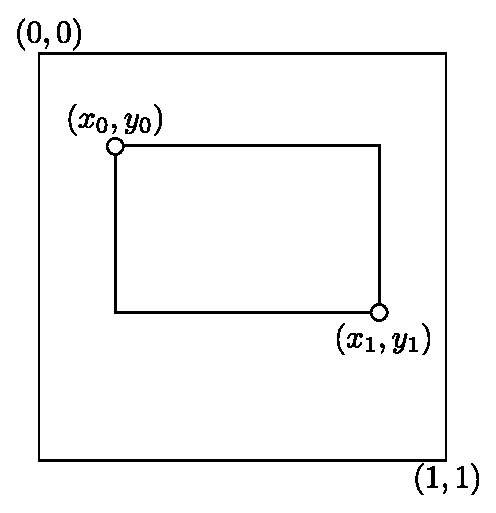
\includegraphics[width=0.4\linewidth]{chap07/Cropwindow.eps}
    \caption{图像裁剪窗口指定要渲染的图像子集。
    它在NDC空间中给出,坐标范围为从$(0,0)$到$(1,1)$.
    类\refvar{Film}{}仅为裁剪窗口内的区域分配空间存储像素值。}
    \label{fig:7.47}
\end{figure}

\refvar[croppedPixelBounds]{Film::croppedPixelBounds}{}保存了
裁剪窗口从左上角到右下角的像素边界。小数像素坐标被舍入;
这保证了如果图像按邻接的裁剪窗口分块渲染,则最终像素只在一个子图像内出现。
\begin{lstlisting}
`\initcode{Compute film image bounds}{=}`
`\refvar{croppedPixelBounds}{}` =
    `\refvar{Bounds2i}{}`(`\refvar{Point2i}{}`(std::ceil(`\refvar{fullResolution}{}`.x * cropWindow.`\refvar{pMin}{}`.x),
                     std::ceil(`\refvar{fullResolution}{}`.y * cropWindow.`\refvar{pMin}{}`.y)),
             `\refvar{Point2i}{}`(std::ceil(`\refvar{fullResolution}{}`.x * cropWindow.`\refvar{pMax}{}`.x),
                     std::ceil(`\refvar{fullResolution}{}`.y * cropWindow.`\refvar{pMax}{}`.y)));
\end{lstlisting}
\begin{lstlisting}
`\refcode{Film Public Data}{+=}\lastcode{FilmPublicData}`
`\refvar{Bounds2i}{}` `\initvar{croppedPixelBounds}{}`;
\end{lstlisting}

有了(可能被裁的)图像像素分辨率后,构造函数
为每个像素分配一个\refvar{Pixel}{}结构体数组。
光谱像素贡献值的滑动加权和用XYZ颜色(\refsub{XYZ颜色})表示
并保存于成员变量\refvar[Pixel::xyz]{xyz}{}中。
\refvar[Pixel::filterWeightSum]{filterWeightSum}{}
持有表示样本对像素的贡献的滤波权重值之和。
\refvar[Pixel::splatXYZ]{splatXYZ}{}持有样本溅射
\sidenote{译者注:此短语翻译不确定,原文sample splats。
目前笔者查阅到splatting一词常译作抛雪球算法。欢迎读者提供帮助。}(不加权)的和。
成员\refvar[Pixel::pad]{pad}{}是没用的;
它唯一的目的是保证结构体\refvar{Pixel}{}是32字节大小,而不是28
(这里假设\refvar{Float}{}是4字节;否则它保证这是64字节结构体)。
该填充保证了\refvar{Pixel}{}不会跨越缓存行,
这样当获取\refvar{Pixel}{}时引发的缓存缺失不超过一次
(只要数组的首个\refvar{Pixel}{}是在缓存行开头分配的)。
\begin{lstlisting}
`\initcode{Film Private Data}{=}\initnext{FilmPrivateData}`
struct `\initvar{Pixel}{}` {
    `\refvar{Float}{}` `\initvar[Pixel::xyz]{xyz}{}`[3] = { 0, 0, 0 };
    `\refvar{Float}{}` `\initvar[Pixel::filterWeightSum]{filterWeightSum}{}` = 0;
    `\refvar{AtomicFloat}{}` `\initvar[Pixel::splatXYZ]{splatXYZ}{}`[3];
    `\refvar{Float}{}` `\initvar[Pixel::pad]{pad}{}`;
};
std::unique_ptr<`\refvar{Pixel}{}`[]> `\initvar[Film::pixels]{pixels}{}`;
\end{lstlisting}
\begin{lstlisting}
`\initcode{Allocate film image storage}{=}`
`\refvar[Film::pixels]{pixels}{}` = std::unique_ptr<`\refvar{Pixel}{}`[]>(new `\refvar{Pixel}{}`[`\refvar{croppedPixelBounds}{}`.Area()]);
\end{lstlisting}

用XYZ颜色存储像素值的两个自然选择是用\refvar{Spectrum}{}值或存储RGB值。
这里即使是进行全光谱渲染也不值得保存完整的\refvar{Spectrum}{}值。
因为写入到输出文件的最终颜色不含\refvar{Spectrum}{}样本全集,
故这里转换为三刺激值和先保存\refvar{Spectrum}{}再转换
为图像输出上的三刺激值相比并不代表损失了信息。
该情况下若\refvar{Spectrum}{}有大量样本,
则不保存完整的\refvar{Spectrum}{}值能节约大量内存
(若pbrt支持把\refvar{SampledSpectrum}{}值保存到文件,则需重新考虑该设计选择)。

我们已选择用XYZ颜色而不是RGB以强调XYZ是独立于显示器的颜色表示,
而RGB需要假定显示器响应曲线的特定集合(\refsub{RGB颜色})。
(然而最后我们还是不得不转换为RGB,因为很少有图像文件格式保存XYZ颜色。)

有了典型的滤波器设置,每个图像样本都可能对最终图像中的16个或更多像素作出贡献。
特别是对于在光线相交测试和着色计算上花费相对较少时间的简单场景,
花在为每个样本更新图像上的时间会很多。
因此,\refvar{Film}{}预先计算滤波值的表使得
我们可以免去对方法\refvar{Filter::Evaluate}{()}的虚函数调用开销
以及推算滤波器的开销,而可以为滤波使用来自表中的值。
实践中因不在每个样本的精确位置上推算滤波而引入的误差并不明显。

这里的实现做了合理假设即滤波器定义满足$f(x,y)=f(|x|,|y|)$,
所以表格只需要为滤波偏移量正\keyindex{象限}{quadrant}{}存储值。
该假设对于目前pbrt中所有可用的\refvar{Filter}{}
都成立且在实践中对大多数滤波器成立。
这让表的大小变为四分之一并改进了内存访问的一致性,
使缓存性能更好\footnote{这里该实现可进一步利用目前pbrt中所有滤波器都是可分离的事实,
只分配两个1D表。然而,为了允许更容易地添加不同滤波函数,我们这里没有假定可分离性。}。
\begin{lstlisting}
`\initcode{Precompute filter weight table}{=}`
int offset = 0;
for (int y = 0; y < `\refvar{filterTableWidth}{}`; ++y) {
    for (int x = 0; x < `\refvar{filterTableWidth}{}`; ++x, ++offset) {
        `\refvar{Point2f}{}` p;
        p.x = (x + 0.5f) * `\refvar{filter}{}`->`\refvar[Filter::radius]{radius}{}`.x / `\refvar{filterTableWidth}{}`;
        p.y = (y + 0.5f) * `\refvar{filter}{}`->`\refvar[Filter::radius]{radius}{}`.y / `\refvar{filterTableWidth}{}`;
        `\refvar[Film::filterTable]{filterTable}{}`[offset] = `\refvar{filter}{}`->`\refvar[Filter::Evaluate]{Evaluate}{}`(p);
    }
}
\end{lstlisting}
\begin{lstlisting}
`\refcode{Film Private Data}{+=}\lastnext{FilmPrivateData}`
static constexpr int `\initvar{filterTableWidth}{}` = 16;
`\refvar{Float}{}` `\initvar[Film::filterTable]{filterTable}{}`[`\refvar{filterTableWidth}{}` * `\refvar{filterTableWidth}{}`];
\end{lstlisting}

\refvar{Film}{}的实现负责确定\refvar{Sampler}{}要
为之生成样本的整数像素值范围。方法
\refvar{GetSampleBounds}{()}返回要采样的区域。
因为像素重建滤波器通常作用于许多像素,所以\refvar{Sampler}{}必须
生成稍微超出实际输出像素范围的图像样本。
这样即使是图像边界上的像素,在所有方向上也有同等密度的样本围绕着它,
而不会因只有来自图像内部方向的值而被偏置。
这一细节在渲染具有裁剪窗口的分块图像时也很重要,因为它消除了子图像边缘的伪影。

计算样本边界涉及将离散转换为连续像素坐标时要考虑的半个像素偏移量,
按滤波器半径扩展,再向外舍入。
\begin{lstlisting}
`\refcode{Film Method Definitions}{+=}\lastnext{FilmMethodDefinitions}`
`\refvar{Bounds2i}{}` `\refvar{Film}{}`::`\initvar{GetSampleBounds}{()}` const {
    `\refvar{Bounds2f}{}` floatBounds(
        `\refvar{Floor}{}`(`\refvar{Point2f}{}`(`\refvar{croppedPixelBounds}{}`.`\refvar{pMin}{}`) + `\refvar{Vector2f}{}`(0.5f, 0.5f) -
              `\refvar{filter}{}`->`\refvar[Filter::radius]{radius}{}`),
        `\refvar{Ceil}{}`( `\refvar{Point2f}{}`(`\refvar{croppedPixelBounds}{}`.`\refvar{pMax}{}`) - `\refvar{Vector2f}{}`(0.5f, 0.5f) +
              `\refvar{filter}{}`->`\refvar[Filter::radius]{radius}{}`));
    return (`\refvar{Bounds2i}{}`)floatBounds;
}
\end{lstlisting}

\refvar{GetPhysicalExtent}{()}返回场景中胶片的实际范围。
\refvar{RealisticCamera}{}尤其需要该信息。
有了胶片对角线长度和图像高宽比,我们可以计算$x$和$y$方向上的传感器尺寸。
如果我们记对角线长度为$d$,胶片传感器的宽和高为$x$和$y$,
则我们知道$x^2+y^2=d^2$.我们可以定义图像的高宽比$a$为$\displaystyle a=\frac{y}{x}$,
则$y=ax$,即得$x^2+a^2x^2=d^2$.求解$x$得
\begin{align*}
    x=\sqrt{\frac{d^2}{1+a^2}}\, .
\end{align*}

下面就是\refvar{GetPhysicalExtent}{()}的实现。返回的范围以$(0,0)$为中心。
\begin{lstlisting}
`\refcode{Film Method Definitions}{+=}\lastnext{FilmMethodDefinitions}`
`\refvar{Bounds2f}{}` `\refvar{Film}{}`::`\initvar{GetPhysicalExtent}{}`() const {
    `\refvar{Float}{}` aspect = (`\refvar{Float}{}`)`\refvar{fullResolution}{}`.y / (`\refvar{Float}{}`)`\refvar{fullResolution}{}`.x;
    `\refvar{Float}{}` x = std::sqrt(`\refvar{diagonal}{}` * `\refvar{diagonal}{}` / (1 + aspect * aspect));
    `\refvar{Float}{}` y = aspect * x;
    return `\refvar{Bounds2f}{}`(`\refvar{Point2f}{}`(-x / 2, -y / 2), `\refvar{Point2f}{}`(x / 2, y / 2));
}
\end{lstlisting}

\subsection{为胶片提供像素值}\label{sub:为胶片提供像素值}
有三种方式可以把样本贡献提供给胶片。
第一种由\refvar{Sampler}{}在图块上生成的样本驱动。
尽管大多数简单接口都允许渲染器提供一个胶片像素位置
以及表示相应光线对\refvar{Film}{}的直接贡献的\refvar{Spectrum}{},
但在多线程情形下要提供这类方法的高性能实现并不容易,
多线程可能最终试图并发地更新图像的同一部分。

因此\refvar{Film}{}定义了能让线程表明其正生成整个图像中某一范围像素的接口。
有了样本边界,\refvar{GetFilmTile}{()}转而返回指向\refvar{FilmTile}{}对象的指针,
它存有图像相应区域中像素的贡献。\refvar{FilmTile}{}的所有权
及其存储的数据只属于调用者,故线程可以给\refvar{FilmTile}{}提供样本值
而不担心和其他线程争夺。当它完成该图块上的工作,
线程就将完整图块回传给\refvar{Film}{},安全地将其合并到最终图像。
\begin{lstlisting}
`\refcode{Film Method Definitions}{+=}\lastnext{FilmMethodDefinitions}`
std::unique_ptr<`\refvar{FilmTile}{}`> `\refvar{Film}{}`::`\initvar{GetFilmTile}{}`(
        const `\refvar{Bounds2i}{}` &sampleBounds) {
    `\refcode{Bound image pixels that samples in sampleBounds contribute to}{}`
    return std::unique_ptr<`\refvar{FilmTile}{}`>(new `\refvar{FilmTile}{}`(tilePixelBounds,
        `\refvar{filter}{}`->`\refvar[Filter::radius]{radius}{}`, `\refvar[Film::filterTable]{filterTable}{}`, `\refvar{filterTableWidth}{}`));
}
\end{lstlisting}

有了将在其中生成样本的像素区域边界框,计算样本值将要贡献的图像像素边界框有两步。
第一,必须考虑离散到连续像素坐标变换的影响以及滤波器半径。
第二,结果的边界必须裁剪到全图像素边界;按照定义不需要考虑图像之外的像素。
\begin{lstlisting}
`\initcode{Bound image pixels that samples in sampleBounds contribute to}{=}`
`\refvar{Vector2f}{}` halfPixel = `\refvar{Vector2f}{}`(0.5f, 0.5f);
`\refvar{Bounds2f}{}` floatBounds = (`\refvar{Bounds2f}{}`)sampleBounds;
`\refvar{Point2i}{}` p0 = (`\refvar{Point2i}{}`)`\refvar{Ceil}{}`(floatBounds.`\refvar{pMin}{}` - halfPixel -
                           `\refvar{filter}{}`->`\refvar[Filter::radius]{radius}{}`);
`\refvar{Point2i}{}` p1 = (`\refvar{Point2i}{}`)`\refvar{Floor}{}`(floatBounds.`\refvar{pMax}{}` - halfPixel +
                            `\refvar{filter}{}`->`\refvar[Filter::radius]{radius}{}`) + `\refvar{Point2i}{}`(1, 1);
`\refvar{Bounds2i}{}` tilePixelBounds =
    `\refvar[Bounds3::Intersect]{Intersect}{}`(`\refvar{Bounds2i}{}`(p0, p1), `\refvar{croppedPixelBounds}{}`);
\end{lstlisting}
\begin{lstlisting}
`\refcode{Film Declarations}{+=}\lastcode{FilmDeclarations}`
class `\initvar{FilmTile}{}` {
public:
    `\refcode{FilmTile Public Methods}{}`
private:
    `\refcode{FilmTile Private Data}{}`
};
\end{lstlisting}

\refvar{FilmTile}{}构造函数接收一个2D边界框,
它给出了最终图像中的像素边界,须为这些像素提供存储和所用重建滤波器的额外信息,
包括指向在{\refcode{Precompute filter weight table}{}}中制成表的滤波函数值的指针。
\begin{lstlisting}
`\initcode{FilmTile Public Methods}{=}\initnext{FilmTilePublicMethods}`
`\refvar{FilmTile}{}`(const `\refvar{Bounds2i}{}` &pixelBounds, const `\refvar{Vector2f}{}` &filterRadius,
    const `\refvar{Float}{}` *filterTable, int filterTableSize)
    : `\refvar{pixelBounds}{}`(pixelBounds), `\refvar{filterRadius}{}`(filterRadius),
    `\refvar{invFilterRadius}{}`(1 / filterRadius.x, 1 / filterRadius.y),
    `\refvar[FilmTile::filterTable]{filterTable}{}`(filterTable), `\refvar{filterTableSize}{}`(filterTableSize) {
    `\refvar[FilmTile::pixels]{pixels}{}` = std::vector<`\refvar{FilmTilePixel}{}`>(std::max(0, pixelBounds.Area()));
}
\end{lstlisting}

\begin{lstlisting}
`\initcode{FilmTile Private Data}{=}`
const `\refvar{Bounds2i}{}` `\initvar{pixelBounds}{}`;
const `\refvar{Vector2f}{}` `\initvar{filterRadius}{}`, `\initvar{invFilterRadius}{}`;
const `\refvar{Float}{}` *`\initvar[FilmTile::filterTable]{filterTable}{}`;
const int `\initvar{filterTableSize}{}`;
std::vector<`\refvar{FilmTilePixel}{}`> `\initvar[FilmTile::pixels]{pixels}{}`;
\end{lstlisting}

对于每个像素,保留来自像素样本的加权贡献之和
(依据重建滤波器权重)以及滤波器权重之和。
\begin{lstlisting}
`\initcode{FilmTilePixel Declarations}{=}`
struct `\initvar{FilmTilePixel}{}` {
    `\refvar{Spectrum}{}` `\initvar[FilmTilePixel::contribSum]{contribSum}{}` = 0.f;
    `\refvar{Float}{}` `\initvar[FilmTilePixel::filterWeightSum]{filterWeightSum}{}` = 0.f;
};
\end{lstlisting}

一旦算出光线为样本所带的辐亮度,\refvar{Integrator}{}就
调用\refvar[AddSample]{FilmTile::AddSample}{()}。
它接收一个样本以及相应的辐亮度值和
\refvar[GenerateRayDifferential]{Camera::GenerateRayDifferential}{()}
原本返回的样本贡献权重。它用重建滤波器和像素滤波方程更新存储的图像。
\begin{lstlisting}
`\refcode{FilmTile Public Methods}{+=}\lastnext{FilmTilePublicMethods}`
void `\initvar{AddSample}{}`(const `\refvar{Point2f}{}` &pFilm, const `\refvar{Spectrum}{}` &L,
    `\refvar{Float}{}` sampleWeight = 1.) {
    `\refcode{Compute sample's raster bounds}{}`
    `\refcode{Loop over filter support and add sample to pixel arrays}{}`
}
\end{lstlisting}

为了理解\refvar[AddSample]{FilmTile::AddSample}{()}的操作,
首先回想像素滤波方程:
\begin{align*}
    I(x,y)=\frac{\sum\limits_i{f(x-x_i,y-y_i)w(x_i,y_i)L(x_i,y_i)}}{\sum\limits_i{f(x-x_i,y-y_i)}}\, .
\end{align*}
它同时用滤波函数$f$和\refvar{Camera}{}返回的样本权重$w(x_i,y_i)$计算
辐亮度值对最终像素值的贡献,把每个像素的值$I(x,y)$算为附近样本辐亮度值的加权和。
因为pbrt中所有\refvar{Filter}{}都具有有限范围,
所以该方法先计算哪些像素将被当前样本影响。
然后它翻转像素滤波方程,为受该样本影响的每个像素$(x,y)$更新两个滑动之和。
一个和累积了像素滤波方程的分子,另一个累积了分母。
在渲染结束时,通过执行除法算得最终像素值。

为了求得一个样本可能对哪些像素有贡献,\refvar[AddSample]{FilmTile::AddSample}{()}通过
从$x$和$y$中减去0.5将连续样本坐标转化为离散坐标。
然后它用每个方向的滤波半径来偏移该值(\reffig{7.48}),
将其变换到图块坐标空间,并对最小坐标向上取整,对最大坐标向下取整,
因为范围边界外的像素不受该样本影响。
最后,该像素边界被裁剪到图块中的像素边界。
尽管理论上该样本可能贡献于图块之外的像素,
但任何这样的像素都一定在图像范围之外。
\begin{figure}[htbp]
    \centering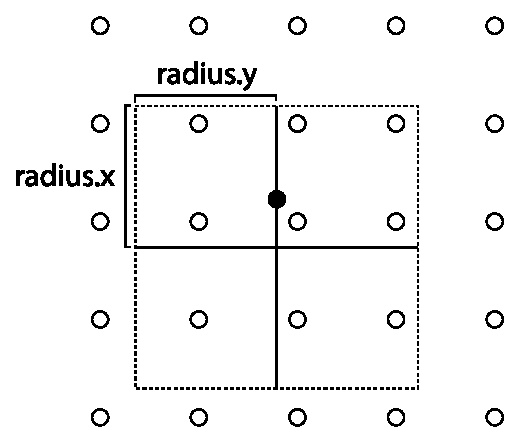
\includegraphics[width=0.5\linewidth]{chap07/Samplepixelcontributions.eps}
    \caption{给定图像平面上某一位置的一个图像样本(实心点),
    必须确定哪些像素值(空心点)会受该样本贡献的影响。
    依据像素重建滤波器半径(实线)取得$x$和$y$方向的偏移量
    并找出该区域内的像素即可完成之。}
    \label{fig:7.48}
\end{figure}

\begin{lstlisting}
`\initcode{Compute sample's raster bounds}{=}`
`\refvar{Point2f}{}` pFilmDiscrete = pFilm - `\refvar{Vector2f}{}`(0.5f, 0.5f);
`\refvar{Point2i}{}` p0 = (`\refvar{Point2i}{}`)`\refvar{Ceil}{}`(pFilmDiscrete - `\refvar{filterRadius}{}`);
`\refvar{Point2i}{}` p1 = (`\refvar{Point2i}{}`)`\refvar{Floor}{}`(pFilmDiscrete + `\refvar{filterRadius}{}`) + `\refvar{Point2i}{}`(1, 1);
p0 = `\refvar[Point3::Max]{Max}{}`(p0, `\refvar{pixelBounds}{}`.`\refvar{pMin}{}`);
p1 = `\refvar[Point3::Min]{Min}{}`(p1, `\refvar{pixelBounds}{}`.`\refvar{pMax}{}`);
\end{lstlisting}

有了受该样本影响的像素边界,现在就能在所有那些像素上循环,
对其每一个都累积滤波后的样本权重。
\begin{lstlisting}
`\initcode{Loop over filter support and add sample to pixel arrays}{=}`
`\refcode{Precompute x and y filter table offsets}{}`
for (int y = p0.y; y < p1.y; ++y) {
    for (int x = p0.x; x < p1.x; ++x) {
        `\refcode{Evaluate filter value at (x,y) pixel}{}`
        `\refcode{Update pixel values with filtered sample contribution}{}`
    }
}
\end{lstlisting}

每个离散整数像素$(x,y)$都有以其为中心的滤波函数实例。
为了给特定样本计算滤波权重,需要在离散坐标中
求出从像素到该样本位置的偏移量并代入滤波函数。
如果我们显式代入滤波器,则合适的计算将是
{\ttfamily\newline\noindent
filterWeight = filter->Evaluate(Point2i(x - pFilmDiscrete.x,\newline\noindent
\indent\indent\indent\indent\indent\indent\indent\indent\indent\indent\quad y - pFilmDiscrete.y));\newline\noindent}
而该实现代之以从表中检索合适的滤波权重。

给定样本位置$(x,y)$,为了给像素$(x',y')$求得滤波权重,
该例程计算偏移量$(x'-x,y'-y)$并将其转化为滤波权重查询表所需的坐标。
这可通过用样本偏移量每个分量除以那个方向的滤波器半径直接做到,
得到在0和1间的值,然后乘以表的大小。注意到沿$x$方向上的每行像素,
其$y$的差,即滤波表中的$y$偏移量,是常数,由此可进一步优化该过程。
类似地,对于每列像素,$x$偏移量也是常数。
因此,这里于像素上循环之前可以预先计算这些索引并将其存入两个1D数组,
节约循环中的重复工作。
\begin{lstlisting}
`\initcode{Precompute x and y filter table offsets}{=}`
int *ifx = `\refvar{ALLOCA}{}`(int, p1.x - p0.x);
for (int x = p0.x; x < p1.x; ++x) {
    `\refvar{Float}{}` fx = std::abs((x - pFilmDiscrete.x) * 
                        `\refvar{invFilterRadius}{}`.x * `\refvar{filterTableSize}{}`);
    ifx[x - p0.x] = std::min((int)std::floor(fx), `\refvar{filterTableSize}{}` - 1);
}
int *ify = `\refvar{ALLOCA}{}`(int, p1.y - p0.y);
for (int y = p0.y; y < p1.y; ++y) {
    `\refvar{Float}{}` fy = std::abs((y - pFilmDiscrete.y) * 
                        `\refvar{invFilterRadius}{}`.y * `\refvar{filterTableSize}{}`);
    ify[y - p0.y] = std::min((int)std::floor(fy), `\refvar{filterTableSize}{}` - 1);
}
\end{lstlisting}

现在对于每个像素,可为其求得滤波表中的$x$和$y$偏移量,
得到对数组的偏移量以及滤波值。
\begin{lstlisting}
`\initcode{Evaluate filter value at (x,y) pixel}{=}`
int offset = ify[y - p0.y] * `\refvar{filterTableSize}{}` + ifx[x - p0.x];
`\refvar{Float}{}` filterWeight = `\refvar[FilmTile::filterTable]{filterTable}{}`[offset];
\end{lstlisting}

对于每个被影响的像素,我们现在可以将其加权的光谱贡献
以及滤波权重加到\refvar[FilmTile::pixels]{pixels}{}数组中的适当值上。
\begin{lstlisting}
`\initcode{Update pixel values with filtered sample contribution}{=}`
`\refvar{FilmTilePixel}{}` &pixel = `\refvar[FilmTilePixel::GetPixel]{GetPixel}{}`(`\refvar{Point2i}{}`(x, y));
pixel.`\refvar[FilmTilePixel::contribSum]{contribSum}{}` += L * sampleWeight * filterWeight;
pixel.`\refvar[FilmTilePixel::filterWeightSum]{filterWeightSum}{}` += filterWeight;
\end{lstlisting}

方法\refvar[FilmTilePixel::GetPixel]{GetPixel}{()}接收相对整幅图像的像素坐标
并在对数组\refvar[FilmTile::pixels]{pixels}{}索引前
将其转化为胶片分块上的坐标。除了这里的版本,
该方法还有返回{\ttfamily const \refvar{FilmTilePixel}{} \&}的{\ttfamily const}变种。
\begin{lstlisting}
`\refcode{FilmTile Public Methods}{+=}\lastnext{FilmTilePublicMethods}`
`\refvar{FilmTilePixel}{}` &`\initvar[FilmTilePixel::GetPixel]{GetPixel}{}`(const `\refvar{Point2i}{}` &p) {
    int width = `\refvar{pixelBounds}{}`.`\refvar{pMax}{}`.x - `\refvar{pixelBounds}{}`.`\refvar{pMin}{}`.x;
    int offset = (p.x - `\refvar{pixelBounds}{}`.`\refvar{pMin}{}`.x) +
                 (p.y - `\refvar{pixelBounds}{}`.`\refvar{pMin}{}`.y) * width;
    return `\refvar[FilmTile::pixels]{pixels}{}`[offset];
}
\end{lstlisting}

渲染进程使用方法\refvar{MergeFilmTile}{()}呈递将要
合并到图像中的\refvar{FilmTile}{},图像由\refvar{Film}{}保存。
其实现先获取互斥锁以保证多个线程不会同时修改图像像素值。
注意到因为\refvar{MergeFilmTile}{()}接收对图块的{\ttfamily std::unique\_ptr},
所以当调用该方法时该图块内存的所有权被转移了。
因此在调用该方法后调用代码不应再试图把贡献加到图块上。
\refvar{MergeFilmTile}{()}执行结束时,
当参数{\ttfamily tile}离开作用域,\refvar{FilmTile}{}的存储被自动释放。
\begin{lstlisting}
`\refcode{Film Method Definitions}{+=}\lastnext{FilmMethodDefinitions}`
void `\refvar{Film}{}`::`\initvar{MergeFilmTile}{}`(std::unique_ptr<`\refvar{FilmTile}{}`> tile) {
    std::lock_guard<std::mutex> lock(`\refvar{mutex}{}`);
    for (`\refvar{Point2i}{}` pixel : tile->`\refvar{GetPixelBounds}{}`()) {
        `\refcode{Merge pixel into Film::pixels}{}`
    }
}
\end{lstlisting}
\begin{lstlisting}
`\refcode{Film Private Data}{+=}\lastnext{FilmPrivateData}`
std::mutex `\initvar{mutex}{}`;
\end{lstlisting}

当把图块的贡献并入最终图像时,调用代码必须能找到该图块有做贡献的像素边界。
\begin{lstlisting}
`\refcode{FilmTile Public Methods}{+=}\lastcode{FilmTilePublicMethods}`
`\refvar{Bounds2i}{}` `\initvar{GetPixelBounds}{}`() const { return `\refvar{pixelBounds}{}`; }
\end{lstlisting}

对于图块中的每个像素,只需要将其贡献并入存于\refvar{Film::pixels}{}的值。
\begin{lstlisting}
`\initcode{Merge pixel into Film::pixels}{=}`
const `\refvar{FilmTilePixel}{}` &tilePixel = tile->`\refvar[FilmTilePixel::GetPixel]{GetPixel}{}`(pixel);
`\refvar{Pixel}{}` &mergePixel = `\refvar[Film::GetPixel]{GetPixel}{}`(pixel);
`\refvar{Float}{}` xyz[3];
tilePixel.`\refvar[FilmTilePixel::contribSum]{contribSum}{}`.`\refvar{ToXYZ}{}`(xyz);
for (int i = 0; i < 3; ++i)
    mergePixel.`\refvar[Pixel::xyz]{xyz}{}`[i] += xyz[i];
mergePixel.`\refvar[Pixel::filterWeightSum]{filterWeightSum}{}` += tilePixel.`\refvar[FilmTilePixel::filterWeightSum]{filterWeightSum}{}`;
\end{lstlisting}
\begin{lstlisting}
`\initcode{Film Private Methods}{=}`
`\refvar{Pixel}{}` &`\initvar[Film::GetPixel]{GetPixel}{}`(const `\refvar{Point2i}{}` &p) {
    int width = `\refvar{croppedPixelBounds}{}`.`\refvar{pMax}{}`.x - `\refvar{croppedPixelBounds}{}`.`\refvar{pMin}{}`.x;
    int offset = (p.x - `\refvar{croppedPixelBounds}{}`.`\refvar{pMin}{}`.x) +
        (p.y - `\refvar{croppedPixelBounds}{}`.`\refvar{pMin}{}`.y) * width;
    return `\refvar[Film::pixels]{pixels}{}`[offset];
}
\end{lstlisting}

能够一次性为整幅图像的所有像素直接提供值对于
某些\refvar{Integrator}{}实现也很有用。
方法\refvar{SetImage}{()}允许这样的操作模式。
注意参数{\ttfamily img}\sidenote{译者注:原文笔误写成{\ttfamily image},
此处已修正为和代码的表述一致。}所指数组的元素数量
应该等于{\ttfamily\refvar{croppedPixelBounds}{}.Area()}。
\refvar{SetImage}{()}的实现很简单即在将其转化为XYZ颜色后复制给出的值。
\begin{lstlisting}
`\refcode{Film Method Definitions}{+=}\lastnext{FilmMethodDefinitions}`
void `\refvar{Film}{}`::`\initvar{SetImage}{}`(const `\refvar{Spectrum}{}` *img) const {
    int nPixels = `\refvar{croppedPixelBounds}{}`.Area();
    for (int i = 0; i < nPixels; ++i) {
        `\refvar{Pixel}{}` &p = `\refvar[Film::pixels]{pixels}{}`[i];
        img[i].`\refvar{ToXYZ}{}`(p.xyz);
        p.`\refvar[Pixel::filterWeightSum]{filterWeightSum}{}` = 1;
        p.`\refvar[Pixel::splatXYZ]{splatXYZ}{}`[0] = p.`\refvar[Pixel::splatXYZ]{splatXYZ}{}`[1] = p.`\refvar[Pixel::splatXYZ]{splatXYZ}{}`[2] = 0;
    }
}
\end{lstlisting}

某些光传输算法(尤其是\refsec{双向路径追踪}介绍的双向路径追踪)
需要把贡献“溅射”\sidenote{译者注:原文splat,如前所述该词翻译不确定,下同。}
到任意像素的能力。最终像素值简单计算为有贡献的溅射之和,而不是其加权均值。
通常,给定像素周围的溅射越多,该像素就越亮。
成员变量\refvar{Pixel::splatXYZ}{}声明为\refvar{AtomicFloat}{}类型,
它允许多线程通过方法\refvar{AddSplat}{()}
并发地更新像素值而不用额外同步。
\begin{lstlisting}
`\refcode{Film Method Definitions}{+=}\lastnext{FilmMethodDefinitions}`
void `\refvar{Film}{}`::`\initvar{AddSplat}{}`(const `\refvar{Point2f}{}` &p, const `\refvar{Spectrum}{}` &v) {
    if (!`\refvar{InsideExclusive}{}`((`\refvar{Point2i}{}`)p, `\refvar{croppedPixelBounds}{}`))
        return;
    `\refvar{Float}{}` xyz[3];
    v.`\refvar{ToXYZ}{}`(xyz);
    `\refvar{Pixel}{}` &pixel = `\refvar[Film::GetPixel]{GetPixel}{}`((`\refvar{Point2i}{}`)p);
    for (int i = 0; i < 3; ++i)
        pixel.`\refvar[Pixel::splatXYZ]{splatXYZ}{}`[i].`\refvar{Add}{}`(xyz[i]);
}
\end{lstlisting}

\subsection{图像输出}\label{sub:图像输出}
\begin{lstlisting}
`\refcode{Film Method Definitions}{+=}\lastcode{FilmMethodDefinitions}`
void `\refvar{Film}{}`::`\initvar[Film::WriteImage]{WriteImage}{}`(`\refvar{Float}{}` splatScale) {
    `\refcode{Convert image to RGB and compute final pixel values}{}`
    `\refcode{Write RGB image}{}`
}
\end{lstlisting}
\begin{lstlisting}
`\refcode{Film Private Data}{+=}\lastcode{FilmPrivateData}`
const `\refvar{Float}{}` `\initvar[Film::scale]{scale}{}`;
\end{lstlisting}